%%%%%%%%%%%%%%%%%%%%%%%%%%%%%%%%%%%%%%%%%%%%%%%%%%
%
%  New template code for TAMU Theses and Dissertations starting Fall 2012.  
%  For more info about this template or the 
%  TAMU LaTeX User's Group, see http://www.howdy.me/.
%
%  Author: Wendy Lynn Turner 
%	 Version 1.0 
%  Last updated 8/5/2012
%
%%%%%%%%%%%%%%%%%%%%%%%%%%%%%%%%%%%%%%%%%%%%%%%%%%%
%%%%%%%%%%%%%%%%%%%%%%%%%%%%%%%%%%%%%%%%%%%%%%%%%%%%%%%%%%%%%%%%%%%%%%
%%                           SECTION IV
%%%%%%%%%%%%%%%%%%%%%%%%%%%%%%%%%%%%%%%%%%%%%%%%%%%%%%%%%%%%%%%%%%%%%

\chapter{\uppercase{Implementation}}

\section{Seismic Volume Data Loading, Distribution and Saving}

As mentioned in chapter 2, seismic 3D volume data is a collection of estimated property values of the Earth's subsurface, obtained through seismic reflection survey and organized in 3D spacing form. It is widely used in energy companies for geophysics analysis, which could conduct more accurate subsurface exploration and exploit. As shown in Figure \ref{seisdata}, the seismic volume data is defined through 3 different directions in 3D space: inline, crossline and timeline. The industry usually stored the data slice by slice along crossline direction and each slice is a inline section, which is also the default data organization format of Seismic Data Analytics SDK. In this case, each inline slice is a single split of the whole dataset.

\begin{figure}[h]
\centering
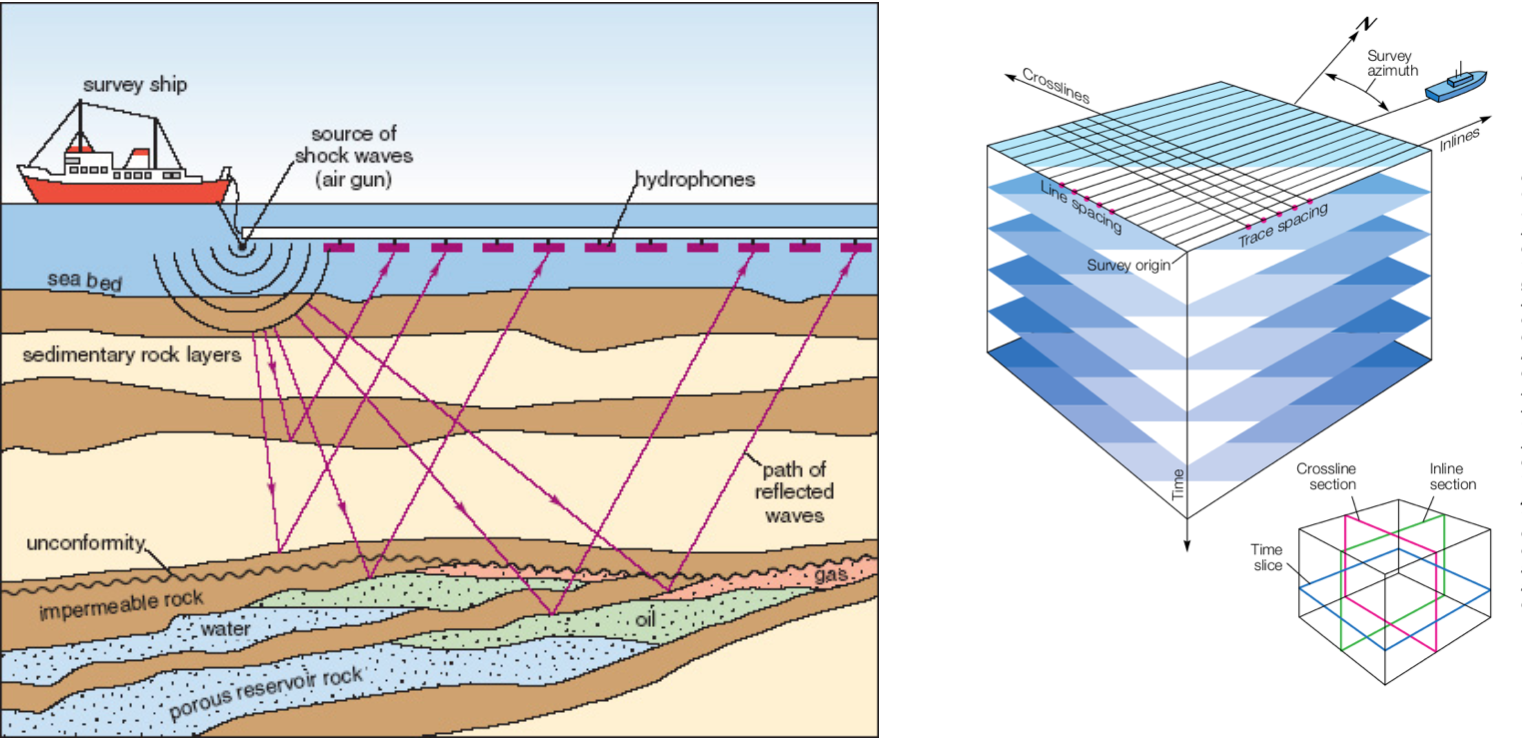
\includegraphics[scale=0.6]{figures/seisdata.png}
\caption{Reflection seismology Survey and Seismic Volume Data \cite{seisaov} \cite{seisinline}}
\label{seisdata}
\end{figure}

The public class \emph{SeismicVolume} provides an API \emph{loadFromFile()} to load seismic data from HDFS and distribute them over Spark RDD according to users configurations. This API generates a \emph{SeismicVolume} instance which contains a SeismicRDD with float/byte as internal binary data types. The SeismicRDD is a derived class from Spark RDD class with a variety of distributed fashions of seismic volume data. In addition, it also provides some optional parameters for advanced users who have already familiar with distributed system to specify the advanced data distribution fashions. 

Figure \ref{datadist} shows the flow of distributing an seismic volume file through the Hadoop filesystem and Spark RDD. It assumes the file has already been uploaded to Hadoop file system, which is able to support the distributed IO accessing for Spark to load data in parallel. After users get the  \emph{SeismicVolume} instance of a specified file,  all Spark RDD operations can be applied to the inside SeismicRDD object. Utilizing the RDD methods provided by Spark, developer could perform various of data operations and calculations on the dataset in parallel. By default, SDK distributes the volume in inline format slice by slice, which means each partition contains one single inline slice. The distribution direction could also be configured to crossline/timeline by given parameters in other APIs, this function will be present in the following Volume Data 3D Transposing section. Users could configure the slices count of each distribution to manage the data distribution grain, thus to efficiently tuning the performance of applications.

\begin{figure}[h]
\centering
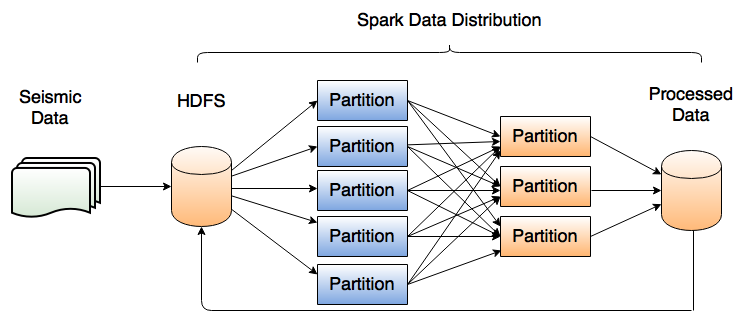
\includegraphics[scale=0.6]{figures/datadist.png}
\caption{Seismic Volume Data Distribution Flow}
\label{datadist}
\end{figure}

\emph{SeismicVolume} class also provides \emph{save()} API to allow users to store the data of SeismicRDD back to the HDFS. Although this operation is not recommended since it could introduce performance issues caused by data shuffling, it is still necessary when users need to backup the runtime data or apply the runtime data to traditional sequential workflows.


\section{Volume Data Accessing}

\begin{figure}[h]
\centering
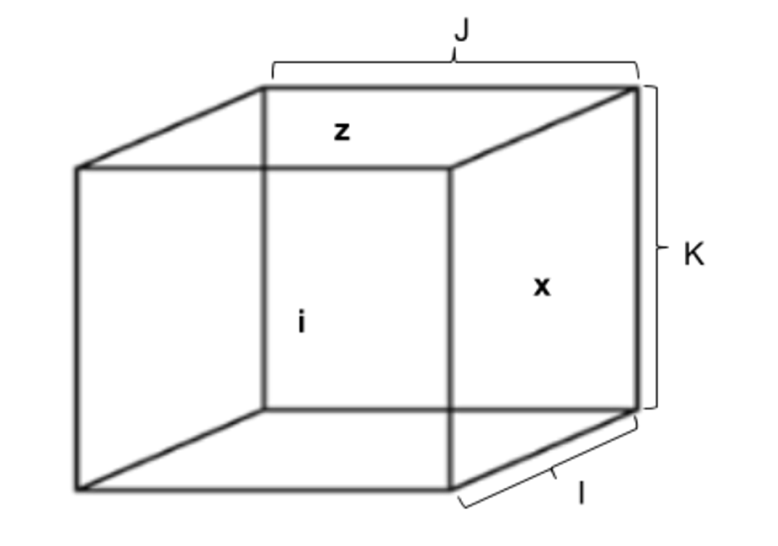
\includegraphics[scale=0.6]{figures/VolumeDim.png}
\caption{Seismic Volume Data Dimensions}
\label{VolumeDim}
\end{figure}

Seismic Data Analytics SDK allows users to to access any slice/trace/sample data in any direction of the volume through \emph{SeismicVolume} APIs \emph{getLine(direction:Int, idx:Int):Array[T]}, \emph{getTrace(dir:Int, i:Int, j:Int):Array[T]} and \emph{getSample(i:Int, j:Int, k:Int):T}. 

For the convenience of addressing the data organization, we defined the three dimension of seismic volume as I (Dimension of inline slices), J (Dimension of crossline slices) and K (Dimension of timeline slices), as shown in Figure \ref{VolumeDim} and Figure \ref{VolumeTrans}. Users can specify any one of I, J and K directions to access data for visualization or computation purpose.  Figure \ref{code_load_access} shows the example of accessing seismic data by \emph{getLine(direction:Int, idx:Int):Array[T]} API. The first parameter of \emph{getLine}, which has three possible direction values(1 stands for I, 2 stands for J and 3 means K), specifies the direction users want to extract the data slice out of.  The second parameter is the index number of the target slice in specified direction.

\begin{figure}[h]
\centering
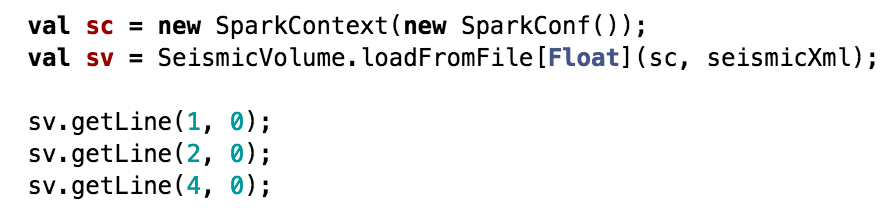
\includegraphics[scale=0.8]{figures/code_load_access.png}
\caption{Example Code of Accessing Data Slice in SeismicVolume}
\label{code_load_access}
\end{figure}


Since Spark does not provide arbitrary data access, the APIs used IndexedRDD, a more efficient key-value management than native Spark API \cite{IndexedRDD}, to implement and speedup queries of slice/trace/sample data from any distributions to the master node.


\section{Volume Data 3D Transposing}

Since the volume data could only be stored in file following one specific direction(I, J or K), developer could not access slices of the other two directions directly. In traditional solutions, if users need data in other directions, organized as cross-line slice or time-line slice, the data fetching program must perform lots of seek operations between different file offsets to collect the data of a single cross-line or time-line slice. This tedious procedure will dramatically slow down the whole software performance. To resolve this problem and to achieve reasonable performance, SDK handles the transposing of the 3D volume data inside the \emph{SeismicVolume} APIs and caches all three directions format SeismicRDD in \emph{SeismicVolume}.

To explain the implementation clearly, we denote the seismic volume data as shown in Figure \ref{VolumeDim}, in which i means I slice, x means J slice and z stands for K slice. The data is stored in iSlices format by default. To resolve the transposing problem in each distribution evenly, we split the volume to I of iSlices and distribute them over SeismicRDD. Each iSlice is a 2D matrix. As shown in Figure \ref{VolumeTrans}, each iSlice matrix consists of J of iTraces which have the length of K. An iSlice matrix could be iterated iTrace by iTrace. Since in 3D spacing, each iTrace is also the trace of xSlice, for example, the iTraces(0) is the xTrace of the 0th xSlice, the iTraces(1) is the xTrace of 1st xSlice, etc. 

As mentioned in previous section, the default distribution of \emph{SeismicVolume} splits the data slice by slice. To transpose the volume data organization to different direction,  first we need to split the slice data partitions to number of smaller trace partitions and index them by trace index number. This process can be achieved by using \emph{flatmap()} operation of Spark RDD. Figure \ref{RDDFlatmap} demonstrates how it splits the data partitions to more fine grain partitions. We apply a map function to \emph{flatmap()} API to index all iTraces of the volume. The new index is combined by index of iTrace and index of iSlice. After indexing the trace map, we got a volume RDD with new (iTraceIndex)(iSliceIndex) index as the key and trace data as the value.

\begin{figure}[h]
\centering
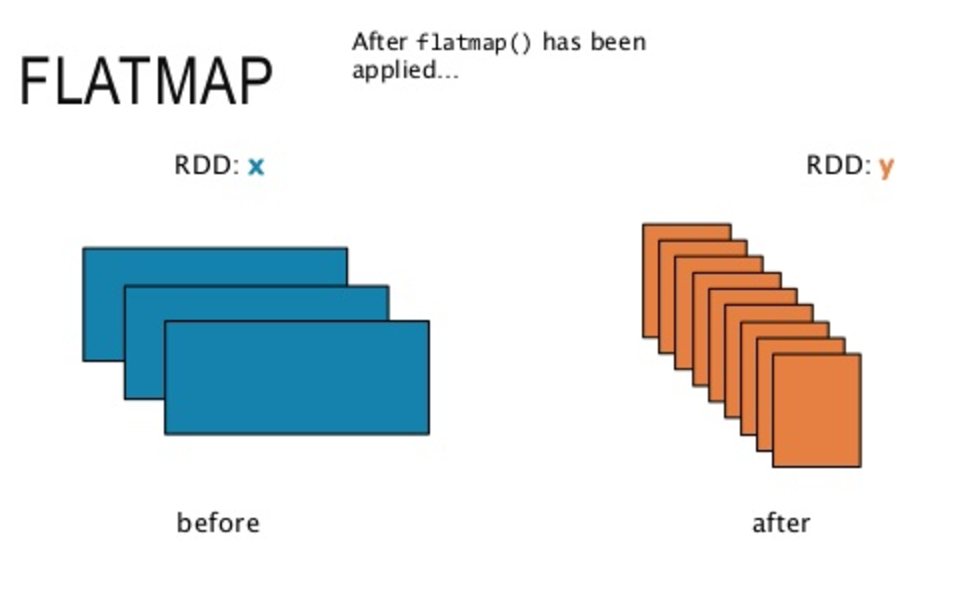
\includegraphics[scale=0.8]{figures/RDDFlatmap.png}
\caption{Flatmap Operation of Spark RDD}
\label{RDDFlatmap}
\end{figure}


As shown in Figure \ref{VolumeTrans}, to get a xSlice, the next step is to group all the traces with the same iTraceIndex by utilizing the \emph{groupByKey} operations of Spark RDD. As shown in Figure \ref{RDDGroup}, this API groups all the data splits sharing the same key feature to a new data partition. After grouping, the xSlices data collection is generated in the new SeismicRDD distribution map. To organize them as a xSlices volume, all we need to do is sorting them by iTraceIndex. So far, the data in requested direction has already been stored in the \emph{SeismicVolume} instance, therefore users could access and manipulate seismic data in any direction by specifying the direction parameter of related \emph{SeismicVolume} APIs.

\begin{figure}[h]
\centering
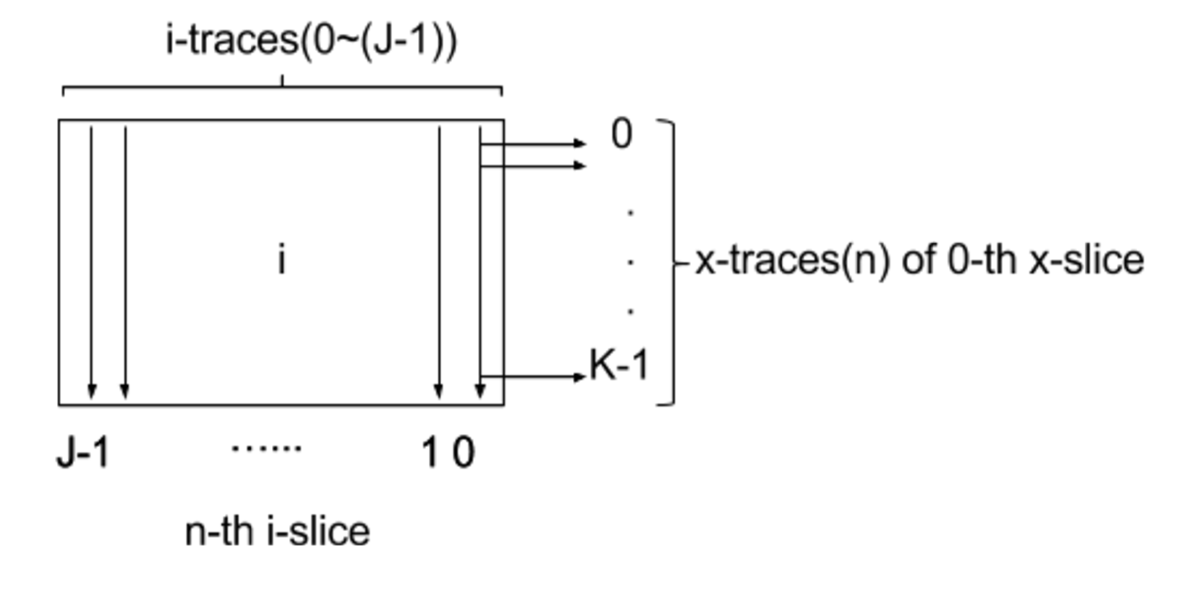
\includegraphics[scale=0.6]{figures/VolumeTrans.png}
\caption{The Indexing for Resolving 3D Transposing Problem}
\label{VolumeTrans}
\end{figure}

\begin{figure}[h]
\centering
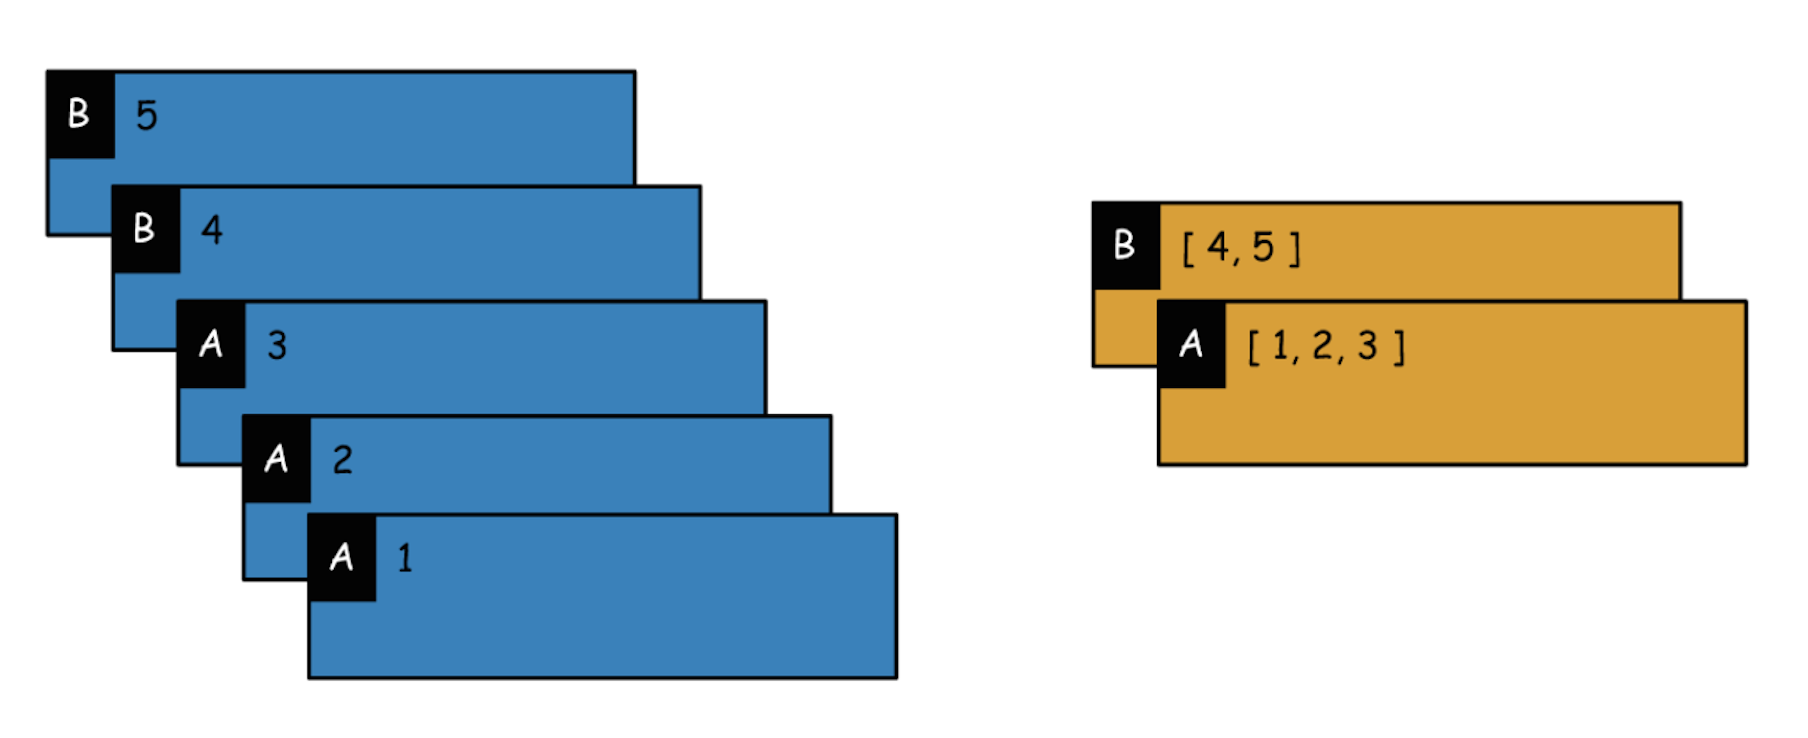
\includegraphics[scale=0.6]{figures/RDDGroup.png}
\caption{GroupByKey Operation of Spark RDD}
\label{RDDGroup}
\end{figure}


\section{Repartition}

Users need a way to configure the data partition size and partitions number, since they need to efficiently tune the granularity of the distributed process to achieve better performance. By default, as shown in Figure \ref{DefDist}, SDK distributes the volume in one specific direction slice by slice. In this case, each slice is a single split of the whole dataset. However, it will cause performance problems for some applications if we only support one distribution. For an instance, the transposing solution as mentioned in previous section needs to do lots of data exchanges between different data splits for the \emph{group} operation to shuffle the dataset to expected arrangement. Since data shuffle in Spark RDD relies on lots of physical storage access and network transmissions in each worker node, it will become the bottleneck of the transposing performance if the number of partitions is too big. Obviously, to speedup the transposing operation, users need to reduce the number of partitions thus to reduce the data communications between worker nodes.

Developers can change the distribution layout to the aggregated and overlapped fashions as shown in Figure \ref{Aggregation} and Figure \ref{Overlap} by utilizing the \emph{SeismicVolume} API :

\emph{repartition(planesPerMap:Int,overlapPlanes:Int):SeismicVolume[T]}.


\subsection{Aggregation}

\begin{figure}[h]
\centering
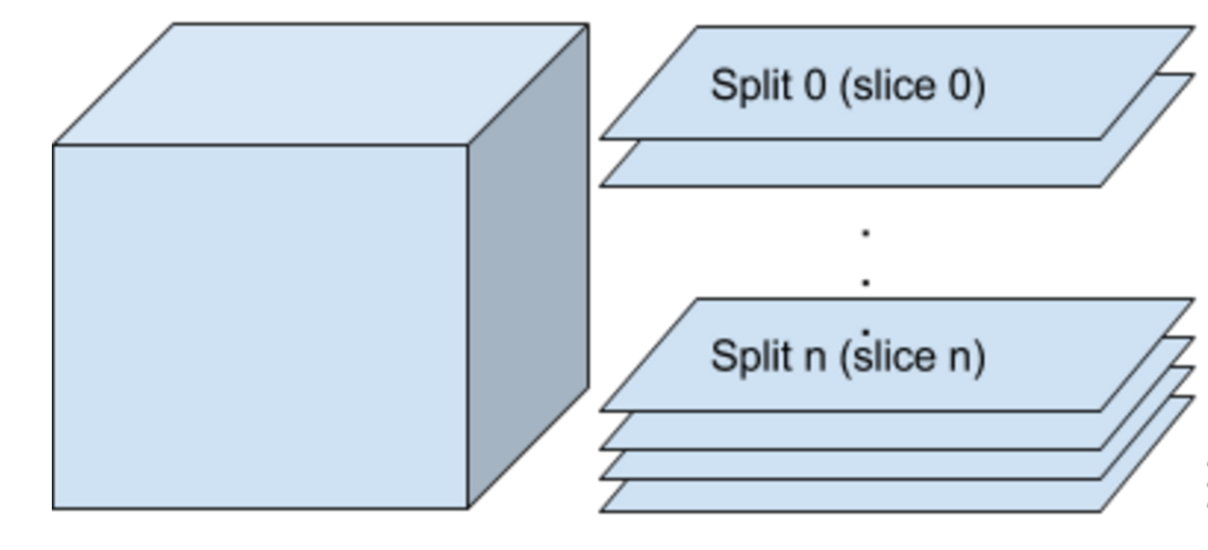
\includegraphics[scale=0.6]{figures/DefDist.png}
\caption{Default Distribution Fashion of Volume, planesPerMap=1, overlap=0}
\label{DefDist}
\end{figure}

As shown in Figure \ref{Aggregation}, aggregated data distribution could be achieved by utilizing the RDD group operations we mentioned in Volume Data 3D transposing section. The solution of this problem is to re-indexing all the slices in parallel through RDD map function by arranging an unique key to multiple data splits, then use RDD \emph{groupByKey()} API to repartition the dataset. An aggregated dataset could have multiple slices in a single data split.

\begin{figure}[h]
\centering
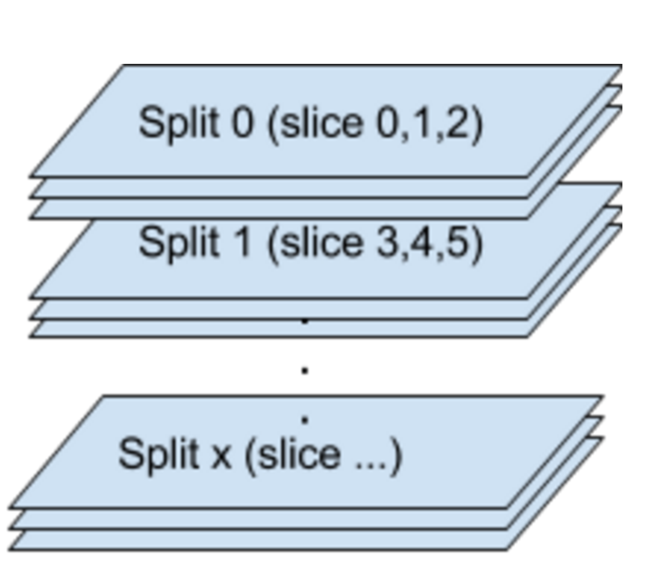
\includegraphics[scale=0.6]{figures/Aggregation.png}
\caption{Aggregated Distribution of Volume, planesPerMap=3, overlap=0}
\label{Aggregation}
\end{figure}

\subsection{Overlapping}

The \emph{repartition()} method not only lets users change the size of distributed splits, more powerfully, it allows developer to set the overlapped data areas between splits and to access the overlapped parts in each split. Practically, some applications may have strong data dependences in their logic which is very hard to parallelize the solutions. For example, the stencil computation needs lots of data communications between neighbor units in each step, which is impossible to run it in parallel with other MapReduce frameworks. 

To resolve this problem, \emph{repartition()} API generates the head and tail boundaries RDD on top of the aggregated SeismicRDD and indexing them according to the related partition numbers. Finally, the boundaries are appended to each related data split through RDD \emph{zip()} API to generate a new \emph{SeismicVolume} instance which contains overlapped SeismicRDD. Figure \ref{boundaryRDD} shows the process of boundary RDD solution.

\begin{figure}[h]
\centering
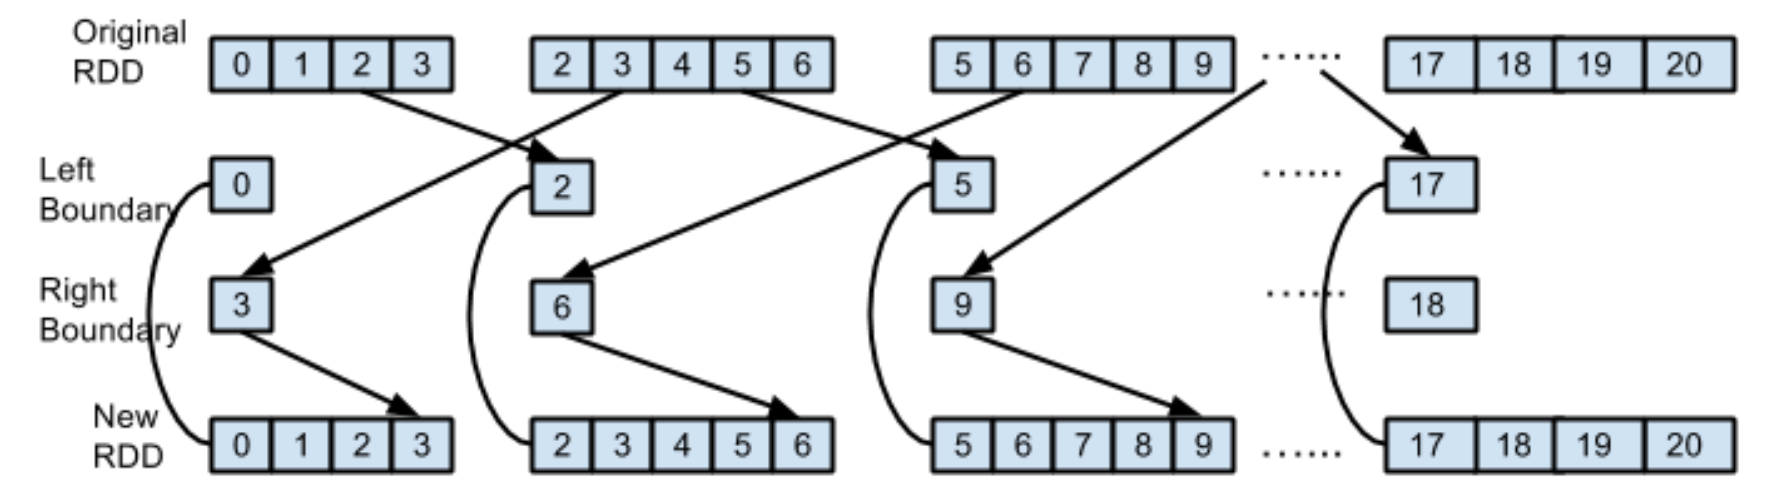
\includegraphics[scale=0.5]{figures/boundaryRDD.png}
\caption{The Boundary RDD Solution of Overlapping Problem}
\label{boundaryRDD}
\end{figure}

\begin{figure}[h]
\centering
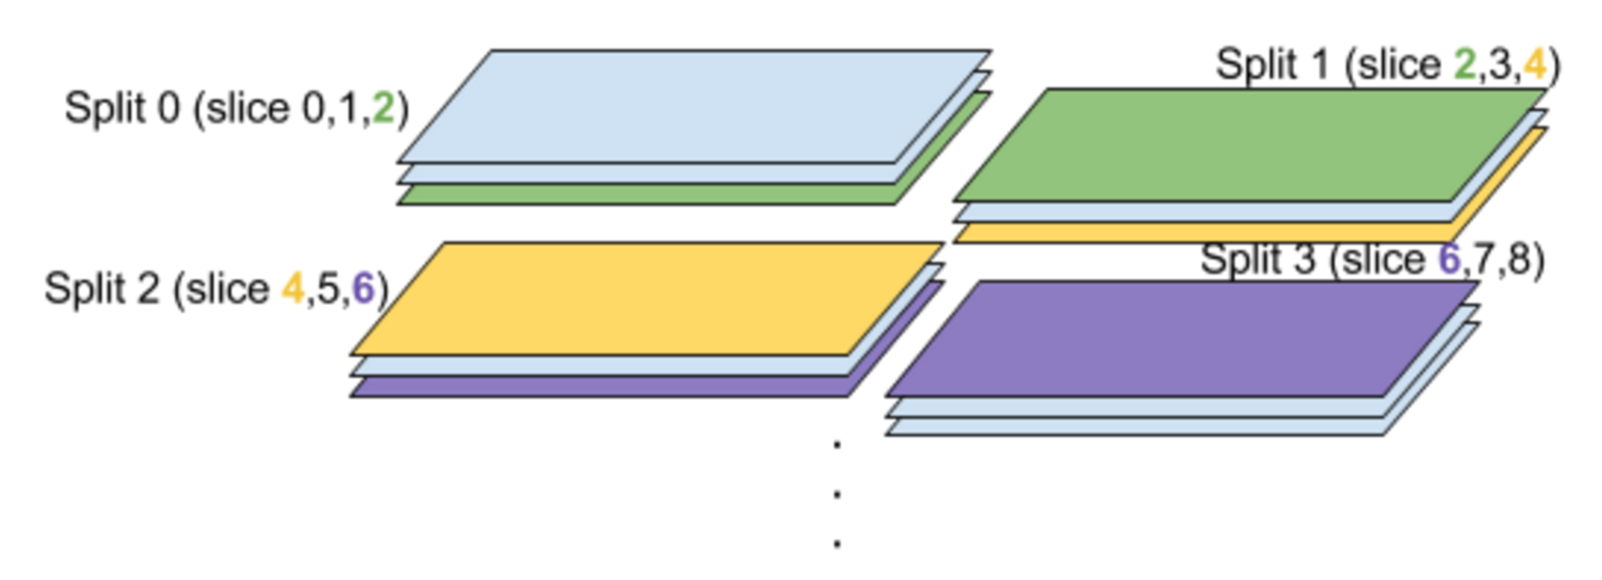
\includegraphics[scale=0.5]{figures/Overlap.png}
\caption{Overlapped distribution of Volume, planesPerMap=1, overlap=1}
\label{Overlap}
\end{figure}

Therefore, this method is not only capable of tuning the performance of distributed tasks, but also simplifies the stencil-style computation requiring neighbor communication, which is not easy to parallelize in MapReduce programming mode. We have developed a more complicated 3D stencil use case with 3D spacing overlapping which will be presented in detail in following Experiments chapter. It could be used for resolving seismic 3D attributes computation problem.


\section{User Defined Function Mapping}

As mentioned in Introduction chapter, one of the project objective is to provide an easy-to-use solution for geophysicists or data scientists to apply their programs on big data platform without concerning the parallelism and code reconstruction. To achieve this, \emph{SeismicVolume} provides \emph{applyMap()} API to allow developer to apply user-defined functions on any direction of the SeismicRDD in parallel. 

The prototype of this API is \emph{applyMap(direction:Int, f:(T-U))}. The first parameter \emph{direction} indicates the direction that users would like to apply the function on. The other parameter \emph{f:(T-U)} is a standard spark RDD key-value pairs operation callback function, which feeds the function distributed volume data with key-value forms in parallel. The data length in each key-value function depends on the specified distribution parameters of the target \emph{SeismicVolume}.  Users could apply any operation or computations on the given input data, and an output key-value pairs is required for the return value. This callback function will be executed along with the related data distribution in parallel. After execution, it will generate a new \emph{SeismicVolume} object containing the processed and distributed dataset output by user-defined function.  Figure \ref{code_apply} shows the example code for users to apply their function.

\begin{figure}[h]
\centering
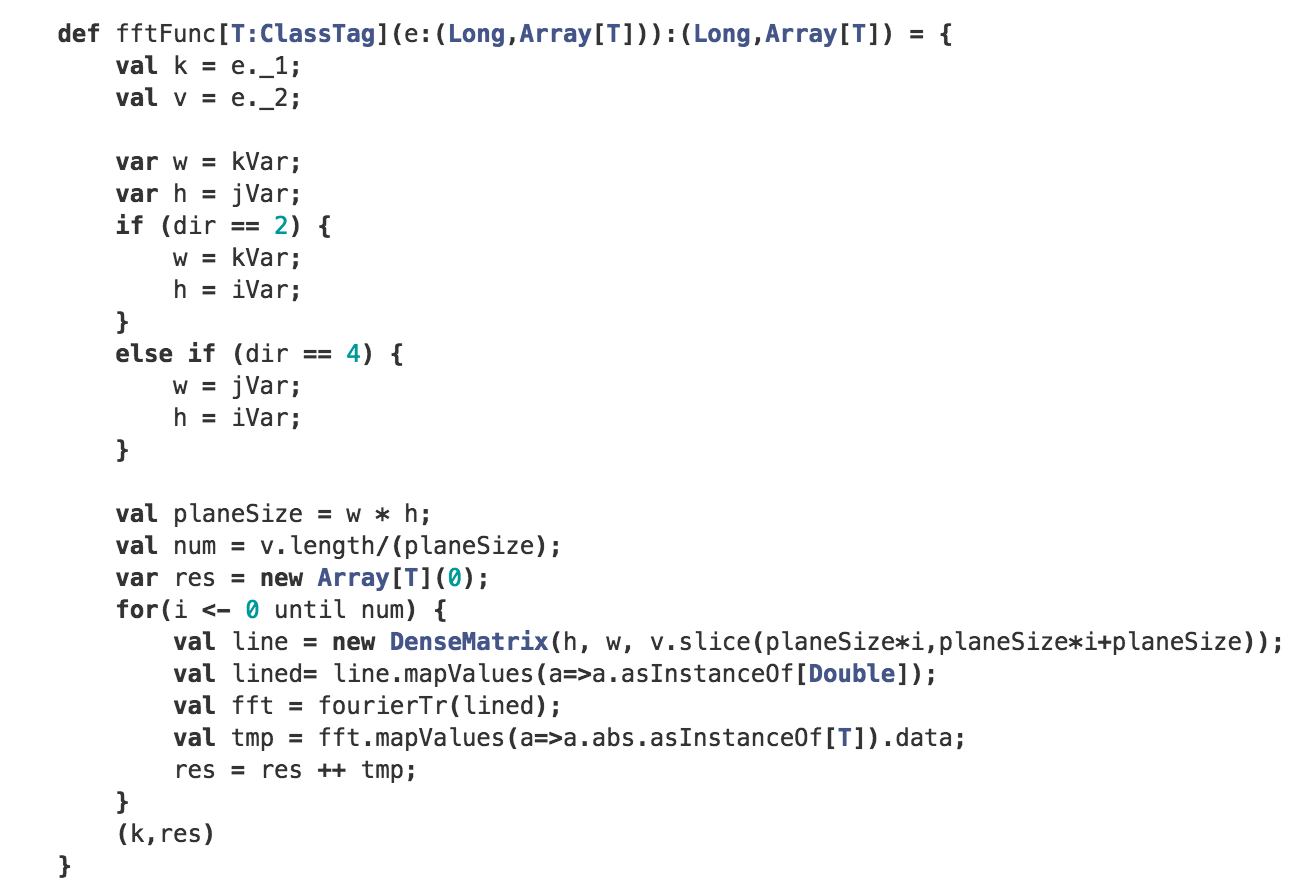
\includegraphics[scale=0.6]{figures/code_apply.png}
\caption{Sample Code for Applying User-defined function in Parallel}
\label{code_apply}
\end{figure}


\section{Parallel Templates}

Data distribution plays an important role in parallel programs to achieve scalable performance. However, most scientists and researchers in petroleum industry do not have enough big data background knowledge to support them to convert their work to Spark applications. To overcome the usability barriers, we developed several parallel templates based on Seismic Data Analytics SDK APIs to make it be easily used by domain algorithm designer other than computer scientists.

These templates defines the data distributions and parallel computation so that users can simply select the right templates for their algorithms without handling the data distribution and parallelism details. Three templates currently include: Trace, Line and Sub-volume. Each template can handle one or more volumes, and will output one or more volumes. Trace template is simple, in which the input is a 2D array (dimension 1 for number of volumes and dimension 2 for 1D trace data), and output is also a 2D array. Line template defines a 3D array as input and a 3D array as output respectively (dimension 1 for number of volumes and dimension 2 for 2D slice data, line is the petroleum terminology). Sub-volume template is a powerful solution to handle data 3D data distribution with overlaps, in which both input and output are 4D array (dimension 1 for number of volumes and dimension 2 for 3D overlapped sub-volume data). The Sub-volume template outputs data without any overlapping. Users can specify parameters about how to distribute data as well as the overlapped areas. 

Figure \ref{code_tmpl_line} shows an example of the Line Template and Figure \ref{code_tmpl_subv} shows the example of Sub-volume Template. Both of them are straight forward and require very few knowledge about parallel computing. The only thing users should be aware of is the distribution grain of input/output data, which is specified in the distribution parameter when users create the template instance. As shown in Figure \ref{code_run_subv}, it demonstrates the execution of an Sub-volume Template instance, in which the distributed input sub-volume size in dimension I and J (for each parallel \emph{proc()} callback function) is set to 26 x 21(The sub-volume size in dimension K is always the complete length of iTrace/xTrace, which is the minimal unit for seismic computation), and the overlapping size is 4 in both I and J direction (Each data split extends to 30 x 25 in I x J). 

\begin{figure}[h]
\centering
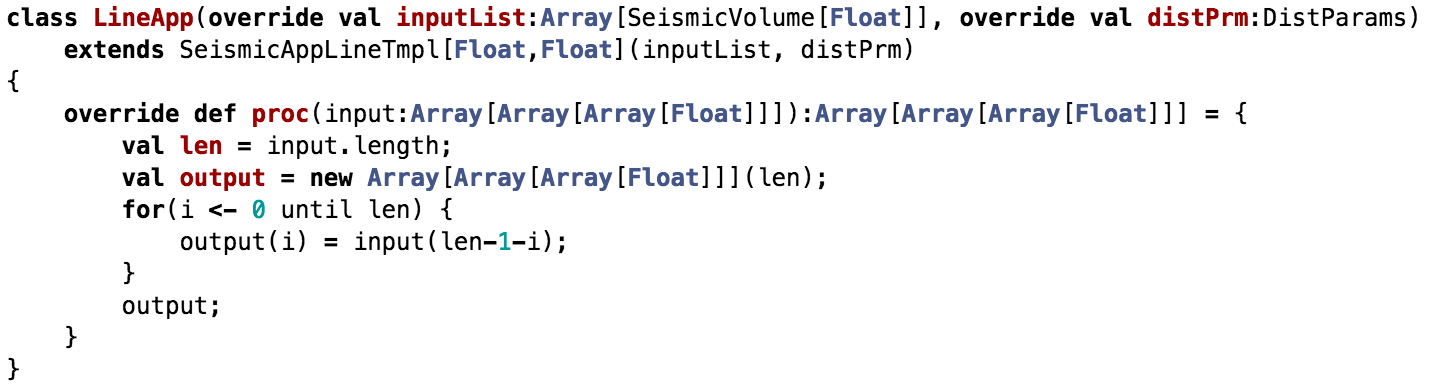
\includegraphics[scale=0.6]{figures/code_tmpl_line.png}
\caption{Sample Code of Line Parallel Template}
\label{code_tmpl_line}
\end{figure}

\begin{figure}[h]
\centering
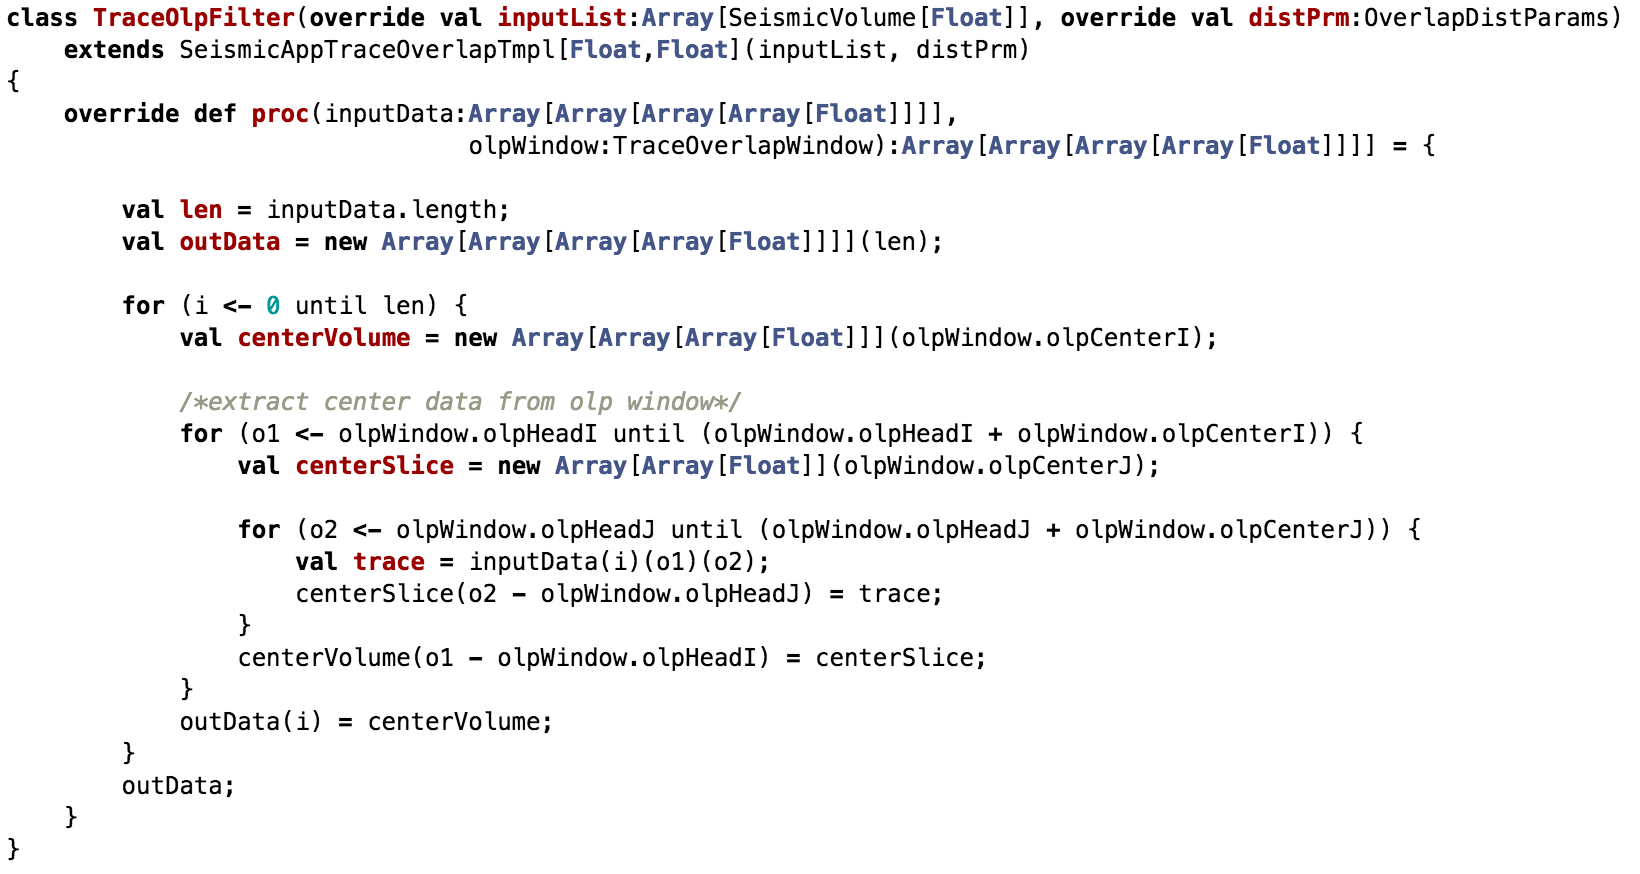
\includegraphics[scale=0.5]{figures/code_tmpl_subv.png}
\caption{Sample Code of Sub-volume Parallel Template}
\label{code_tmpl_subv}
\end{figure}

\begin{figure}[h]
\centering
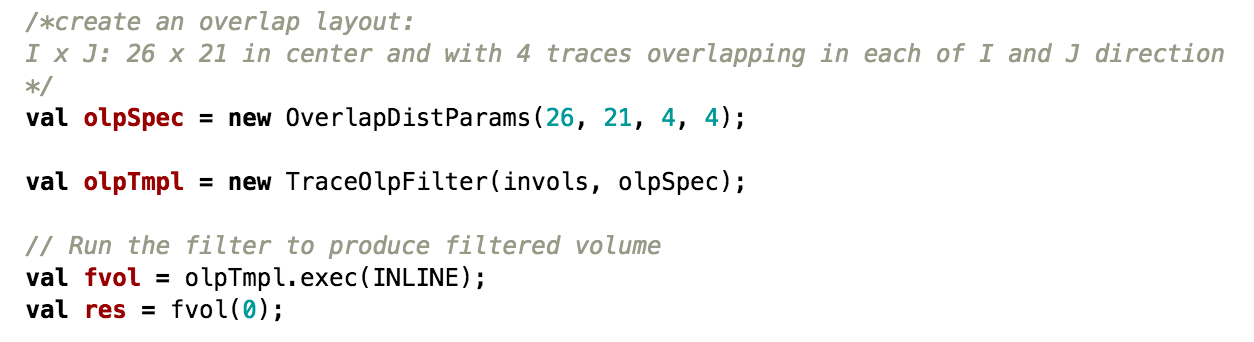
\includegraphics[scale=0.6]{figures/code_run_subv.png}
\caption{Sample Code of Executing Sub-volume Parallel Template}
\label{code_run_subv}
\end{figure}


